\subsubsection*{Design}
\begin{itemize}
	\item As seen in \cref{img:coredes} the core will consist of memory, an ALU combined with the Blitter, and several smaller cores.
	\item The memory is split up into two major parts. The first consists of the double frame buffer, keeping track of the information needed to draw a frame, while the second part is the object memory for the Blitter.
	\item As the functions of the Blitter correlate with the functions of an ALU, we decided to merge them into one. The ALU/Blitter is the only part of the core that is allowed to read and write to the memory.
	\item The smaller cores consist of the graphical functions. These are the two variations of the Bresenham Algorithm, and the function of filling a rectangle.
	\item For the CPU to communicate with the core memory mapped registers are going to be used.
\end{itemize}

\begin{figure}[H]
	\centering
	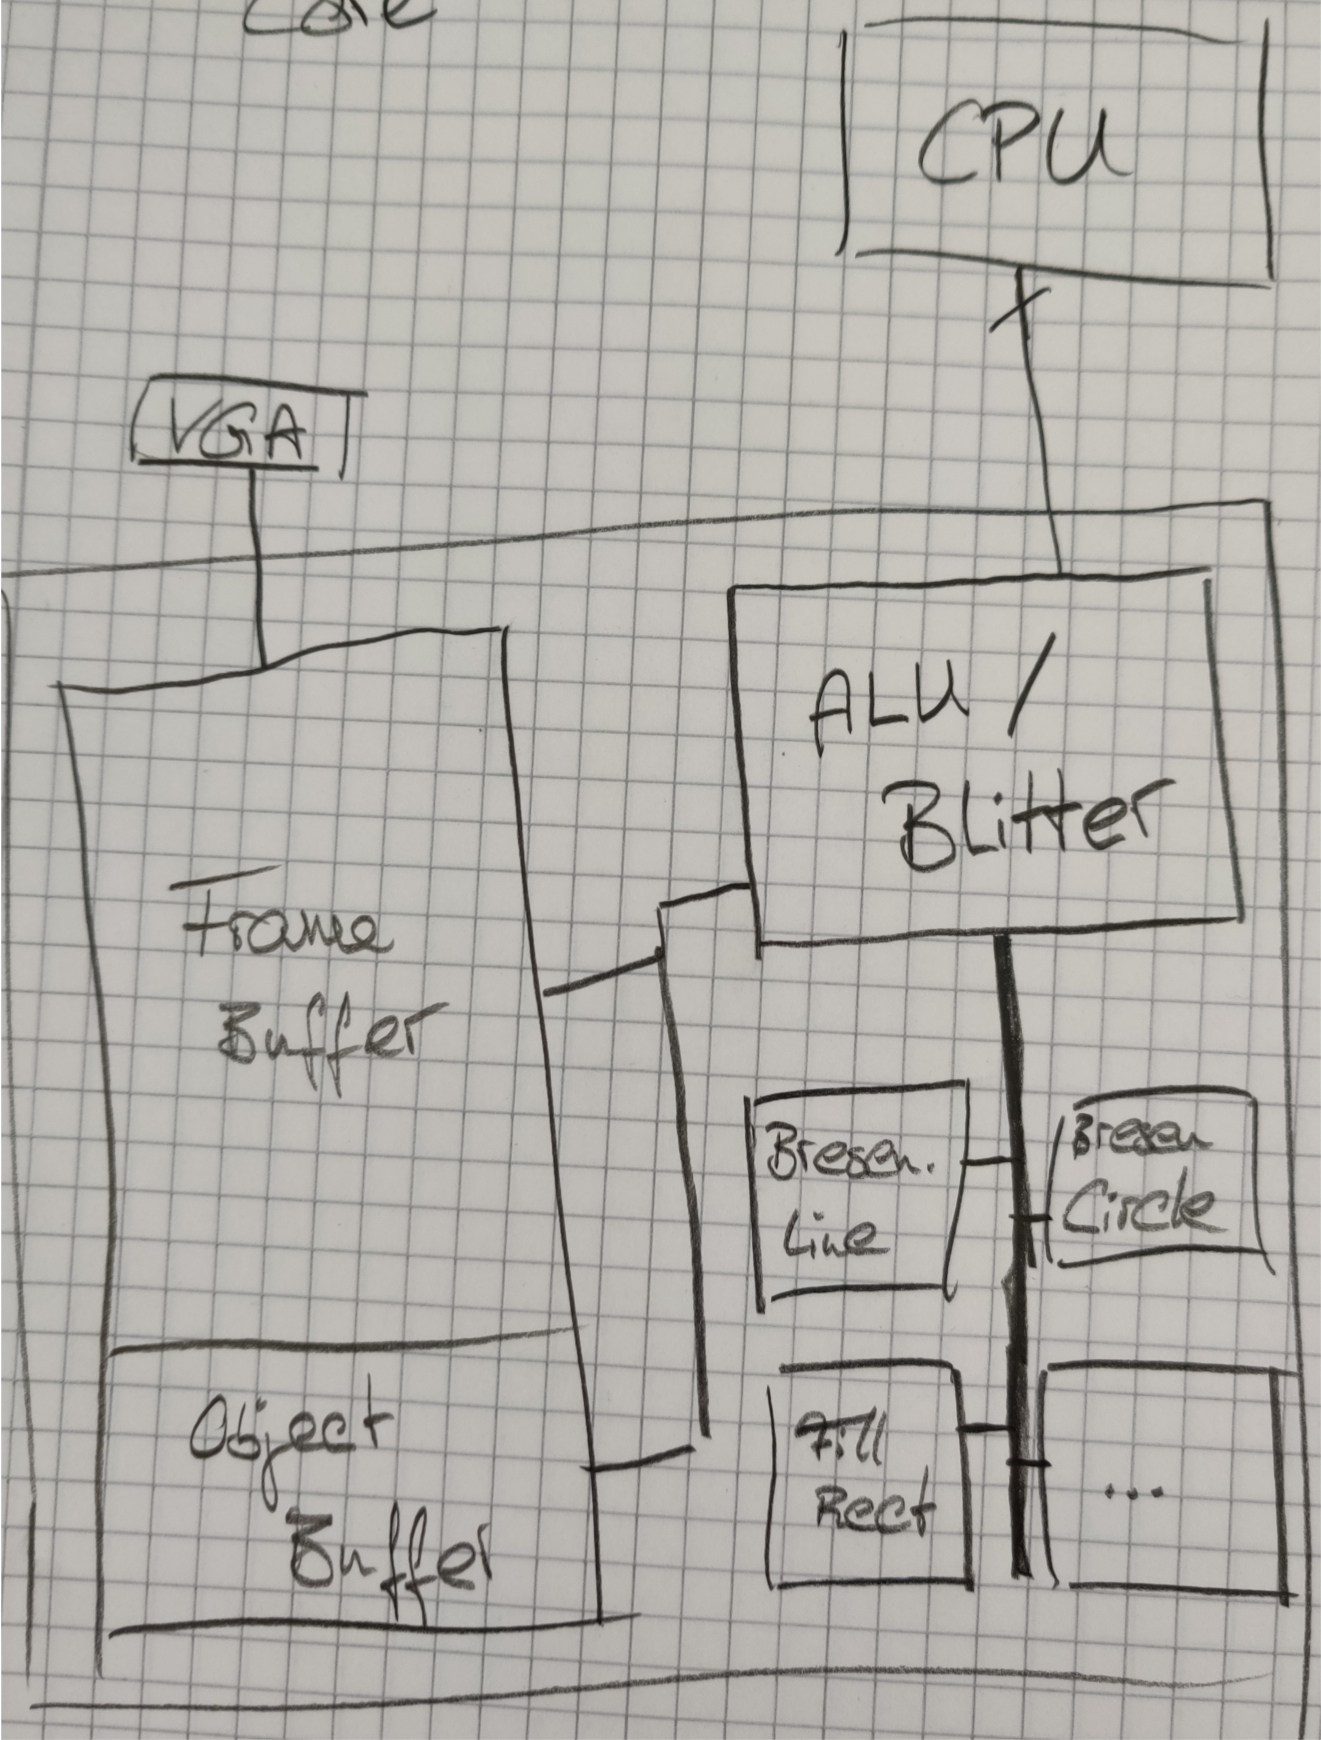
\includegraphics[width=0.5\textwidth]{pre_coredesign}
	\caption{Graphical Design of the AEGIS Core (PLACEHOLDER)}
	\label{img:coredes}
\end{figure}
